\solution:
       The normal equation for the side $AB$ is
\begin{align}
\vec{n}^{\top}\myvec{\vec{x}-\vec{A}}&=0\\
\implies
\vec{n}^{\top}\vec{x}&=\vec{n}^{\top}\vec{A}
\end{align}
Now our task is to find the $\vec{n}$ so that we can find $\vec{n}^{\top}$.
As given in the question 
\begin{align}
  \vec{n} &= \myvec{0 & 1\\
  -1 & 0}\vec{m}
\end{align}
Here $\vec{m} = \vec{B}- \vec{A}$ for side $\vec{AB}$
\begin{align}
\implies
\vec{m}&=\myvec{3\\-5} - \myvec{-3\\-5}\\
&=\myvec{6\\0}
\end{align}
Now as we have obtained vector $\vec{m}$.
we can use this to obtain vector $\vec{n}$
\begin{align}
\vec{n} &= \myvec{0 & 1\\
  -1 & 0}\myvec{6\\0}
 = \myvec{0\\-6}
\end{align}
The transpose of $\vec{n}$ is
\begin{align}
  \vec{n}^{\top}&=\myvec{0 & -6}
\end{align}
Hence the normal equation of side $AB$ is 
\begin{align}
    \myvec{0 & -6}\vec{x}&=\myvec{0 & -6}\myvec{-3\\-5}\\
    \implies
    \myvec{0 & -6}\vec{x}&=30
\end{align}
\begin{figure}
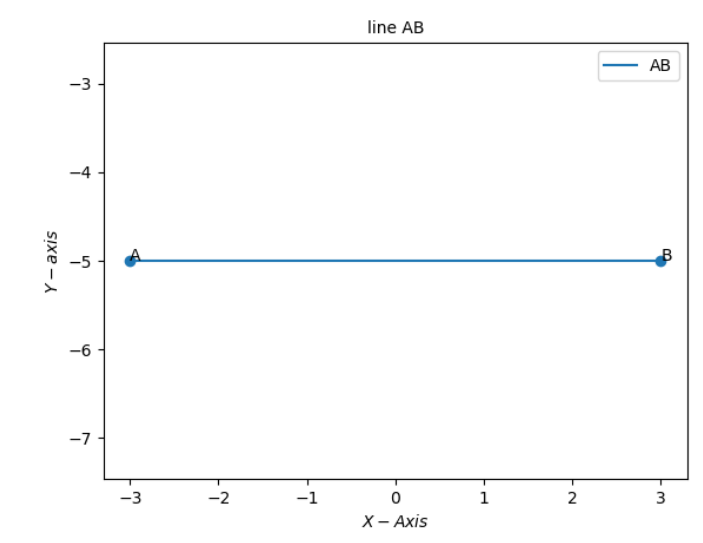
\includegraphics [width=\columnwidth] {figs/lineab.png}
\caption{ The line $\vec{AB}$ plotted using python}
\label{fig: lineab}
\end{figure}


       The normal equation for the side $BC$ is
\begin{align}
\vec{n}^{\top}\myvec{\vec{x}-\vec{B}}&=0\\
\implies
\vec{n}^{\top}\vec{x}&=\vec{n}^{\top}\vec{B}
\end{align}
Now our task is to find the $\vec{n}$ so that we can find $\vec{n}^{\top}$.
As given in the question 
\begin{align}
  \vec{n} &= \myvec{0 & 1\\
  -1 & 0}\vec{m}
\end{align}
Here $\vec{m} = \vec{C}- \vec{B}$ for side $\vec{BC}$
\begin{align}
\implies
\vec{m}&=\myvec{-4\\-3} - \myvec{3\\-5}\\
&=\myvec{-7\\2}
\end{align}
Now as we have obtained vector $\vec{m}$.
we can use this to obtain vector $\vec{n}$
\begin{align}
\vec{n} &= \myvec{0 & 1\\
  -1 & 0}\myvec{-7\\2}
 = \myvec{2\\7}
\end{align}
The transpose of $\vec{n}$ is
\begin{align}
  \vec{n}^{\top}&=\myvec{2 & 7}
\end{align}
Hence the normal equation of side $BC$ is 
\begin{align}
    \myvec{2 & 7}\vec{x}&=\myvec{2 & 7}\myvec{3\\-5}\\
    \implies
    \myvec{2 & 7}\vec{x}&=-29
\end{align}
\begin{figure}
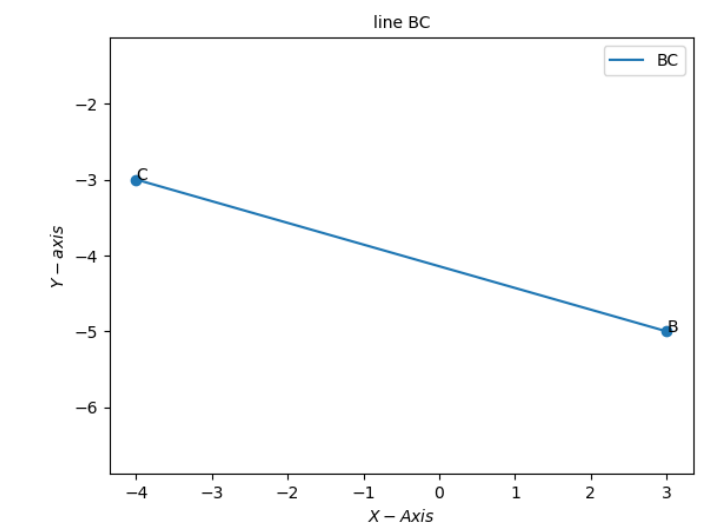
\includegraphics [width=\columnwidth] {figs/linebc.png}
\caption{ The line $\vec{BC}$ plotted using python}
\label{fig: linebc}
\end{figure}



       The normal equation for the side $CA$ is
\begin{align}
\vec{n}^{\top}\myvec{\vec{x}-\vec{C}}&=0\\
\implies
\vec{n}^{\top}\vec{x}&=\vec{n}^{\top}\vec{C}
\end{align}
Now our task is to find the $\vec{n}$ so that we can find $\vec{n}^{\top}$.
As given in the question 
\begin{align}
  \vec{n} &= \myvec{0 & 1\\
  -1 & 0}\vec{m}
\end{align}
Here $\vec{m} = \vec{A}- \vec{C}$ for side $\vec{CA}$
\begin{align}
\implies
\vec{m}&=\myvec{-3\\-5} - \myvec{-4\\-3}\\
&=\myvec{1\\-2}
\end{align}
Now as we have obtained vector $\vec{m}$.
we can use this to obtain vector $\vec{n}$
\begin{align}
\vec{n} &= \myvec{0 & 1\\
  -1 & 0}\myvec{1\\-2}
 = \myvec{-2\\-1}
\end{align}
The transpose of $\vec{n}$ is
\begin{align}
  \vec{n}^{\top}&=\myvec{-2 & -1}
\end{align}
Hence the normal equation of side $CA$ is 
\begin{align}
    \myvec{-2 & -1}\vec{x}&=\myvec{-2 & -1}\myvec{-4\\-3}\\
    \implies
    \myvec{-2 & -1}\vec{x}&=11
\end{align}
\begin{figure}
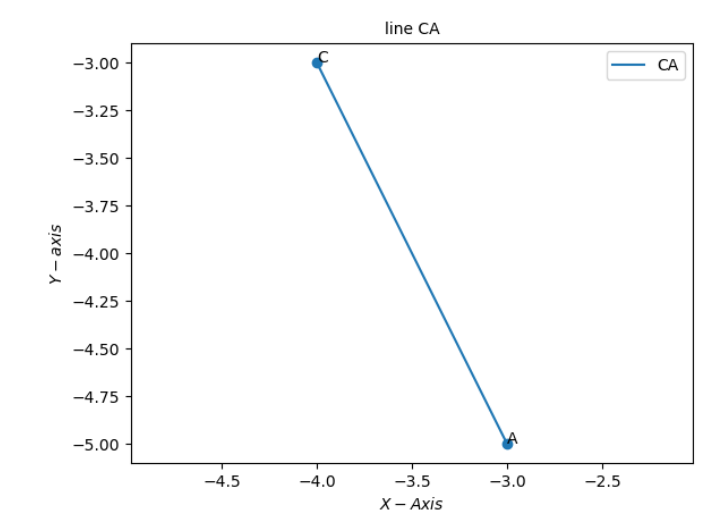
\includegraphics [width=\columnwidth] {figs/lineca.png}
\caption{ The line $\vec{CA}$ plotted using python}
\label{fig: lineca}
\end{figure}